\begin{figure}[!t]
  \centering
  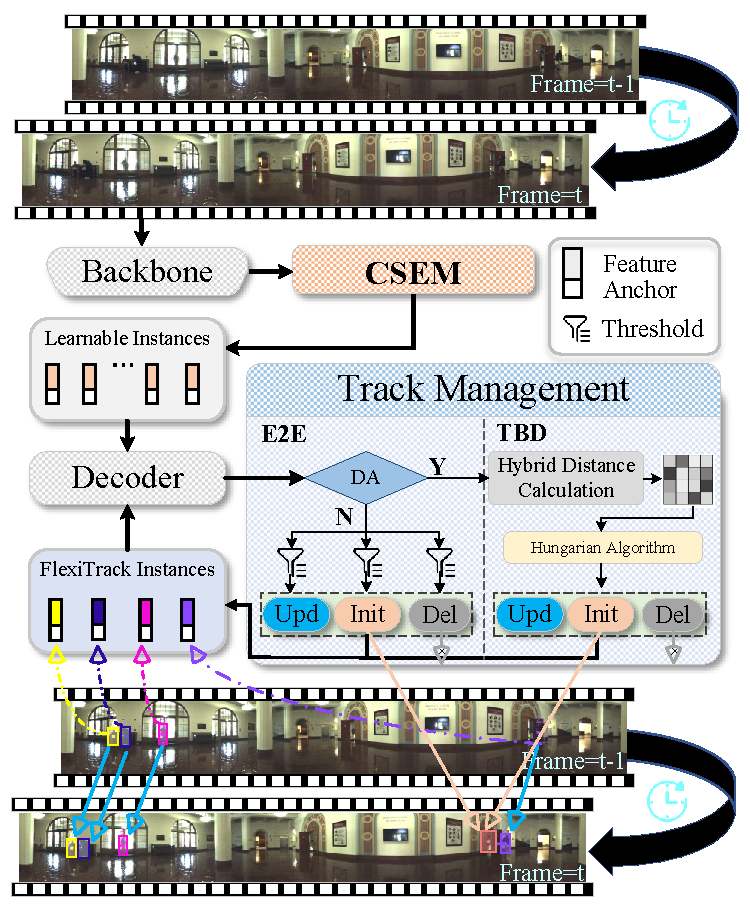
\includegraphics[width=0.48\textwidth]{imgs/id_assignment_single_v2.pdf}
  \vskip -1ex
  \caption{The proposed OmniTrack pipeline. \textbf{CSEM} refers to the CircularStatE Module \ref{subsec:CSEM}
, \textbf{DA} stands for data association, \textbf{E2E} denotes the End-to-End tracking paradigm, \textbf{TBD} refers to the Track-By-Detection tracking paradigm, \textbf{Upd} refers to updating tracks, \textbf{Init} to initializing tracks, and \textbf{Del} to deleting tracks.}

  \label{fig:pipeline}
  \vskip -2ex
\end{figure}

\begin{algorithm}
\caption{OmniTrack Inference Process}
\algorithmfootnote{In \textcolor{codegreen}{green} is the key of our method. }

\label{alg:Omnitrack}
\footnotesize
\KwIn{
A Panoramic video/image sequence $\texttt{V}$
%
}

\KwOut{
Tracks $\mathcal{T}$ of the video/image sequence
%
}

Initialization: $\mathcal{T} \leftarrow \emptyset$\;

Define the Initialize threshold $\mathcal{\tau}_\mathcal{I}$ \;
Define the Update threshold  $\mathcal{\tau}_\mathcal{U}$ \;


\For{frame $f_k$ in $\texttt{V}$}{
\tcc{As shown in Fig. \ref{fig:pipeline}}

$\{\mathcal{S}_3, \mathcal{S}_4, \mathcal{S}_5\} \leftarrow \texttt{Backbone}(f_k)$ \;

\textcolor{codegreen}{$ \mathcal{I}_L \leftarrow  \texttt{CSEM}(\{\mathcal{S}_3, \mathcal{S}_4, \mathcal{S}_5\})$} \;

\textcolor{codegreen}{$ \mathcal{I}_F \leftarrow  \mathcal{T}_{f_{k-1}}$} \;

$ \textcolor{codegreen}{\mathcal{D}_k^F}, \mathcal{D}_k^L \leftarrow  \texttt{Decoder} ( \textcolor{codegreen}{\mathcal{I}_F}, \mathcal{I}_L) $ \;

\BlankLine
\BlankLine
    \If{$\texttt{DA}$}{
        \tcc{Data Association}
	
        $\mathcal{C} \leftarrow  \texttt{Distance Calculation}(\textcolor{codegreen}{{\mathcal{D}_k^F}}+ \mathcal{D}_k^L, \mathcal{T}_{f_{k-1}})$ \;

        $\{\texttt{Update, Initialize, Delate} \} \leftarrow \texttt{Hungarian Algorithm}(\mathcal{C})$ \;
    
        $\mathcal{T}_{f_{k}} \leftarrow \{\texttt{Update, Initialize, Delete} \} $
    }
    
    \Else{
        \tcc{End-to-End}
        
            \textcolor{codegreen}{\For{$d$ in $ \{\mathcal{D}_k^F \cup \mathcal{D}_k^L$\} }{
	            \If{$ d \in \mathcal{D}_k^F \And d.score > \mathcal{\tau}_\mathcal{U} $}{
	               $\texttt{Update} \leftarrow  d$ \;
                }
                    \If{$ d \in \mathcal{D}_k^L \And d.score > \mathcal{\tau}_\mathcal{I}  $}{
	               $\texttt{Initialize } \leftarrow  d$ \;
                }
                \Else{
                    $\texttt{Delete} \leftarrow  d$ \;
                }
            }
        }
        $\mathcal{T}_{f_{k}} \leftarrow \{\texttt{Update, Initialize, Delete} \} $
    }
}


\textbf{Return}: $\mathcal{T}$

%

%
\end{algorithm}

\section{OmniTrack: Proposed Framework}
%

In this section, we introduce OmniTrack, a panoramic multi-object tracking framework that addresses the unique challenges in panoramic-FoV images, including extensive search spaces, geometric distortion, resolution loss, and lighting inconsistencies. 
OmniTrack is designed with a feedback mechanism to iteratively refine object detection, integrating trajectory information back into the detector to enhance tracking stability across panoramic-FoV scenes (Sec.~\ref{subsec:Framework}).
%
Specifically, we propose the OmniTrack framework, which consists of three key components:

%
\begin{itemize}
    \item \textbf{Tracklets Management} (Sec.~\ref{subsec:Tracklets Management}): Manages object trajectory lifecycles and provides temporal priors to the perception module.
    \item \textbf{FlexiTrack Instance} (Sec.~\ref{subsec:Temporal Query}): Rapidly locates and associates objects across the panoramic view by leveraging temporal context.
    \item \textbf{CircularStatE Module} (Sec.~\ref{subsec:CSEM}): Mitigates geometric distortion and improves consistency across the panoramic FoV, enhancing feature reliability.
\end{itemize}

%
\subsection{Feedback Mechanism}
\label{subsec:Framework}
%

The OmniTrack framework, illustrated in Fig.~\ref{fig:pipeline}, incorporates a feedback mechanism that iteratively refines detections by integrating trajectory information back into the detector. This mechanism operates on the principle of reducing information entropy, thereby enhancing stability in Panoramic-FoV and improving MOT performance.

%

In traditional MOT~\cite{zhang2022bytetrack,cao2023observation,du2023strongsort,aharon2022bot}, detection and association are decoupled, leading to higher entropy as each frame’s detection \( H(x_t) \) is calculated independently:
\begin{align}
H(x_t) = -\sum_{i=1}^{n} P(x_t^i) \log P(x_t^i),
\end{align}
where \( x_t^i \) denotes the position of the \( i \)-th target in frame \( t \), with probability distribution \( P(x_t^i) \). The global association entropy~\(H(\{y_t\}) \) depends on the joint probability distribution of target positions across all frames:
\begin{align}
H(\{y_t\}) = -\sum_{i=1}^{n} &P(\{x_1^i, x_2^i, \dots, x_T^i\}) \notag  \\ \times  & \log P(\{x_1^i, x_2^i, \dots, x_T^i\}). 
\label{eq:2}
\end{align} 
The cumulative entropy across all frames, accounting for independent matching, is formulated as:
\begin{align}
H_{\text{independent}} = \sum_{t=1}^{T} H(x_t) + H(\{y_t\}).
\end{align}
%
In contrast, OmniTrack’s feedback mechanism allows detections from frame \( t{-}1 \) to inform those in frame \( t \), reducing per-frame uncertainty. Specifically, the conditional entropy of frame \( t \), given prior feedback \( y_{t-1} \), is:
\begin{align}
H(x_t | y_{t-1}) = -\sum_{i=1}^{n} P(x_t^i | y_{t-1}^i) \log P(x_t^i | y_{t-1}^i).
\end{align}
The total entropy with feedback becomes:
\begin{align}
H_{\text{feedback}} = \sum_{t=1}^{T} H(x_t | y_{t-1}),
\end{align}
where \( H_{\text{feedback}} {<} H_{\text{independent}} \), indicating a reduction in uncertainty over time. This feedback-driven approach thus enhances tracking stability in panoramic-FoV scenarios. 

%

\label{subsec:Mamba encoder}
\begin{figure}[!t]
  \centering
  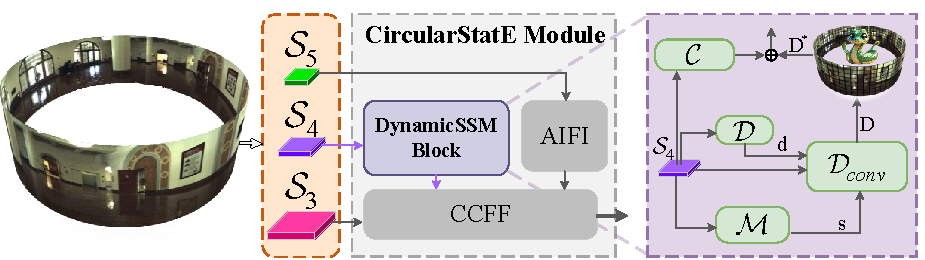
\includegraphics[width=0.48\textwidth]{imgs/CircularStatE_ModuleV4.pdf}
  \caption{The proposed \textbf{CircularStatE Module} fuses multi-scale features to generate learnable instances. The \textbf{DynamicSSM Block} mitigates distortions in panoramic-FoV images, enhancing feature stability across uneven lighting and color distributions.}
  \label{fig: CircularStatE Module}
  \vskip -2ex
\end{figure} 

\subsection{Tracklets Management}
\label{subsec:Tracklets Management}

%

To reduce uncertainty in target localization and association while incorporating temporal information, OmniTrack incorporates a Tracklets Management module. 
During training, this module caches temporal data for instances with confidence scores exceeding a threshold \(\tau\), providing historical context to improve detection consistency in subsequent frames.
During inference, Tracklets Management oversees trajectory lifecycle management by updating, deleting, or initializing instances based on their confidence scores. In scenarios without data association, trajectories are managed directly, forming OmniTrack\(_{E2E}\) (Alg.~\ref{alg:Omnitrack}, Lines 14-21). When data association is enabled, Tracklets Management utilizes TBD-based methods~\cite{cao2023observation,yang2024hybrid} to enhance tracking, referred to as OmniTrack\(_{DA}\) (Alg.~\ref{alg:Omnitrack}, Lines 10-12)

%

\subsection{FlexiTrack Instance}
\label{subsec:Temporal Query}
As described in Eq.~(\ref{eq:2}), the global association entropy is significantly high under panoramic-FoV conditions, making the association task challenging. 
%
Benefiting from the Feedback Mechanism~(Sec.~\ref{subsec:Framework}), which integrates trajectory information into the detector to reduce information entropy.
%
This approach eliminates the need for global search across the entire field of view, making it especially effective for panoramic-scale perception tasks.
Based on this insight, we introduce \emph{FlexiTrack Instance}.

%

Each FlexiTrack Instance (see Fig.~\ref{fig:pipeline}) shares the Decoder network structure with Learnable Instances, consisting of a feature vector \( \mathcal{X} {\in} \mathbb{R}^{128} \) and an anchor \( \mathcal{Y} {\in} \mathbb{R}^{128} \), as shown in Fig.~\ref{fig:pipeline}. 
By sharing the decoder, FlexiTrack Instances can seamlessly adapt to various MOT paradigms, enhancing flexibility and allowing integration across different approaches without additional modifications.
%
To enhance robustness, noise is added to both feature vectors and anchors during training, minimizing dependency on historical data and improving generalization:
\begin{align}
\mathcal{X}' = \mathcal{X} + \mathcal{N}_X, \quad \mathcal{Y}' = \mathcal{Y} + \mathcal{N}_Y, 
\end{align}
where \( \mathcal{N}_X \) and \( \mathcal{N}_Y \) represent the noise components added to the feature vector and anchor, respectively.
To initialize all FlexiTrack Instances, let \( \mathcal{I_F} \) denote the set of initial \emph{instances}, and \( N \) the total number of trajectories. 
Each instance \( \mathcal{I_F}^i \) is composed of a feature vector \( \mathcal{X}_i \) and an anchor \( \mathcal{Y}_i \), as:
\begin{align}
\mathcal{I_F} = \left\{  \mathcal{I_F} ^i \mid \mathcal{I_F}^i = (\mathcal{X}'_i, \mathcal{Y}'_i), i \in \{1, 2, \dots, N\} \right\}.
\end{align}
%
\( \mathcal{X}'_i {\in} \mathbb{R}^{d_{\mathcal{X}}} \) and \( \mathcal{Y}'_i {\in} \mathbb{R}^{d_{\mathcal{Y}}} \) are the feature vector and anchor of the \( i \)-th trajectory, 
%
with \( d_{\mathcal{X}} {=} d_{\mathcal{Y}} {=} 128 \) representing their respective dimensions.
This enables $\mathcal{I_F}$ to inherit trajectory information, guiding the perception module to quickly locate the object and establish temporal associations.

%


% 

\begin{table*}
	\centering
	\small
	\resizebox{0.98\textwidth}{!}{
		\setlength\tabcolsep{8pt}
		\renewcommand\arraystretch{1.0}
    \begin{tabular}{l|cc|cc|cccc}
        % \toprule
        % \hline
        \topline
        \rowcolor{mygray}
          & \multicolumn{2}{c|}{\textbf{Data}} & \multicolumn{2}{c|}{\textbf{Domain}}   & &&&\\
        % \cline{2-4}
        % \hspace{2pt}\cline{2-4}\hspace{2pt}
        
        % \cmidrule(lr){2-4}\cmidrule(lr){5-6}
        % \shortcline{2-4}
        \rowcolor{mygray}
          \multirow{-2}{*}{ \textbf{Datasets}}   &  \textbf{Cov.}  & \textbf{Pano.}  & \textbf{Platform}  & \textbf{Movement}  &  \multirow{-2}{*}{\textbf{Trk Len}} & \multirow{-2}{*}
        {\textbf{No. Seq}} &\multirow{-2}{*}{\textbf{No. Smp}} &\multirow{-2}{*}{\textbf{No. T}} \\
               

        % \midrule 
        \hline\hline
        
 \textbf{KITTI MOT} \cite{geiger2013vision}                  &   \textit{n.a.}   & \crossmark &  \car & \wheels &  \textit{n.a.}  &  21    &   8k       &  749       \\
 %
  \textbf{Waymo}  \cite{waymo}                   &  220$^{\circ}$ & \crossmark &  \car &  \wheels  & 20s & 103k     &      20m       &     \textit{n.a.}    \\
  \textbf{nuScenes}  \cite{caesar2020nuscenes}       &             360$^{\circ}$    & \crossmark & \car  & \wheels &  20s &   1000   &     40k  & \textit{n.a.}    \\
   \textbf{BDD100K MOT}  \cite{bdd100k}               &    \textit{n.a.}  & \crossmark &  \car  &  \wheels & 40s  &   2000   &        398k     &    \textit{n.a.}    \\
   
     \textbf{SportsMOT}   \cite{cui2023sportsmot}               &    \textit{n.a.}  & \crossmark &  \webm & \stationary    & \textit{n.a.} &   240   &      150k       &   3401      \\
     \textbf{DanceTrack}   \cite{peize2021dance}               &  \textit{n.a.}    & \crossmark &  \webm &  \stationary   & \textit{n.a.}  &  100    &      105k       & 990       \\

     \textbf{JRDB} \cite{martin2021jrdb}                  &  360$^{\circ}$    & \crossmark &  \robot &  \wheels  &  $\leq$117s &   54   &      20k       &     \textit{n.a.}    \\
    \textbf{MOT17}   \cite{milan2016mot16}              &   \textit{n.a.}   & \crossmark &  \webm & \gait \stationary   & $\leq$85s  &   14   &       11k      &  1331       \\
    \textbf{MOT20}  \cite{dendorfer2020mot20}              &  \textit{n.a.}    & \crossmark &  \webm & \stationary    & $\leq$133s &   8   &    13k     & 3833   \\
           % \midrule 
           \hline
    \rowcolor{tabgray} \textbf{QuadTrack (ours)}                &   360°    &  \mycheckmark  & \robotdog  &  \gait   &   60s &     32 &       19k      &    332     \\    
        % \bottomrule
        \bottomline
        % \hline
        
    \end{tabular}
	}
 \vspace{-3mm}
	\captionsetup{font=small}
	\caption{Typical datasets for 2D tracking. Abbreviations:  \car~(Autonomous Car), \robot~(Mobile Robot), \robotdog~(Quadruped Robot), \mywebm~(Internet images/videos), \wheels~(Wheels), \gait~(Gait), \stationary~(Stationary), Cov. (Coverage), Pano. (Panoramic camera), %
 Trk Len (Track Length), No. Seq (The number of sequences), No. Smp (The number of samples), and No. T (the number of tracks).}
        \vspace{-3mm}
	\label{tab:comparison dataset}
	\vspace{-8pt}
\end{table*}

%

\subsection{CircularStatE Module} 
\label{subsec:CSEM}
%

The panoramic image provides an exceptionally panoramic FoV, capable of capturing 360{\textdegree} scenes. However, this inevitably introduces issues such as geometric distortions and inconsistencies in color and brightness in real-world high-dynamic-range scenes. To address these challenges, this paper proposes the \emph{CircularStatE Module}, which alleviates distortions and improves the consistency of image features, thereby enhancing the performance of perception models.

%

The \emph{DynamicSSM Block}, which is central to the \emph{CircularStatE Module}, is responsible for mitigating distortions and refining the feature map. The operation is broken down into the following steps: 
\label{mod:DynamicSSM}

\noindent \textbf{Distortion and Scale Calculation.} The first step is to compute both the {distortion} and {scale} information from the input feature map \( S_4 \):
\begin{align}
\mathbf{d}, \mathbf{s} = \mathcal{D}(S_4), \, \sigma(\mathcal{M}(S_4)),
\end{align}
where, \( \mathbf{d} \) and \( \mathbf{s} \) represent the distortion and scale, respectively, both of which have dimensions \( \mathbb{R}^{B \times C \times W \times H} \).

\noindent \textbf{Mitigate Distortion.} To correct distortions, we apply a dynamic convolution \( \mathcal{D}_{conv} \) to refine the feature map. The operation can be expressed as:
\begin{align}
\mathbf{D} = \mathcal{D}_{conv}(\mathbf{d} \odot \mathbf{s}, S_4),
\end{align}
where the symbol $\odot$ represents the Hadamard product, ensuring effective integration of scale adjustments.

\noindent \textbf{Improve Consistency.}
%
Following distortion correction, a State Space Model (SSM) \cite{mamba2} is applied to enhance light and color consistency in the panoramic image. The input to this step is the output from the previous stage, denoted as \(\mathbf{D}{\in}\mathbb{R}^{B\times C\times W\times H}\), and can be represented as follows:
\begin{align}
{\mathbf{D^\ast}}[b,c,x,y]=\frac{1}{N}\sum_{d\in\{scan\}}F_{S6}(S_d(\mathbf{D}[b,c,x,y])),
\end{align}
where \(N\) represents the number of scans, \(S_d\) represents the scanning function, and \(F_{S6}\) is the transformation function for the S6 block \cite{mamba2}.

\noindent \textbf{Feature Fusion.}
Finally, the outputs from the dynamic convolution branch and the residual branch are fused. The fusion module \( \mathcal{F} \) combines the refined feature map \( {\mathbf{D^\ast}}\) with a processed version of \( S_4 \) (obtained via a CNN operation \( \mathcal{C}(S_4) \)) to yield the final output feature map \( \mathbf{F} \):
\begin{align}
\mathbf{F} = \mathcal{F}(\mathcal{C}(S_4) \oplus {\mathbf{D^\ast}}).
\end{align}
\( \oplus \) denotes the feature fusion operation, combining details from both branches for optimal feature representation.

%